\documentclass[../../main.tex]{subfiles}

\begin{document}
\graphicspath{{img/}{05_software/img/}}

\chapter{Thực hiện Gmapping trên nền tảng CUDA}


Bài toán: Giả sử có $N$ particles, mỗi particle biểu diễn một trạng thái của robot bao gồm tọa độ x,y, góc quay theta $(x, y, \theta)^T$ và một map $m_n$ tương ứng với trạng thái đó. Với mỗi bộ dữ liệu đầu vào bao gồm ranging data và odometry data, ta cần dự đoán trạng thái mới của robot đồng thời tiếp tục cập nhật map của môi trường xung quanh.

Nội dung chương phân tích quá trình implement GMapping để giải quyết bài toán trên theo các bước cơ bản của Particle Filter.

\section{Dự đoán - Prediction}
Ở bước này, trạng thái tiếp theo của các particle được tính dựa vào motion model cung cấp từ odometry system. 
\begin{equation}
    \begin{pmatrix}
        \hat{x} \\ \hat{y} \\ \hat{\theta}
    \end{pmatrix}
    = 
    \begin{pmatrix}
        x \\ y \\ \theta
    \end{pmatrix}
    + 
    \begin{pmatrix}
        dx \\ dy \\ d\theta
    \end{pmatrix}
\end{equation}
Với $dx$, $dy$, $d\theta$ có được bằng cách lấy hiệu của trạng thái cung cấp từ odometry hiện giờ và vòng lặp trước.

\section{Hiệu chỉnh - Correction}
Particle filter không có bước này nhưng nó lại giữ một vai trò quan trọng để tăng độ chính xác của thuật toán, nhất là khi có nhiều nhiễu trong quá trình di chuyển của mobile robot hoặc tần số  chạy thuật toán thấp.

Để thực hiện corection, ta sử dụng thuật toán IPC (iterative closest point). Một cách ngắn gọn có thể mô tả thuật toán này như sau:
\begin{itemize}
    \item Với vị trí hiện tại của robot, ta tính toán vị trí của các điểm cuối (vị trí mà các tia laser va vào vật) từ ranging data.
    \item Với mỗi điểm cuối, ta tìm một điểm tương ứng trên map
    \item Sử dụng công thức để tìm biến đổi trung bình từ tập các điểm cuối đến các điểm tương ứng trên map.
    \item Áp dụng phép biến đổi đó vào vị trí hiện tại của robot ta được vị trí mới.
    \item Tiếp tục quay lại bước đầu cho đến khi vị trí robot hầu như không thay đổi nữa hoặc quá một số lượng vòng lặp giới hạn nhất định.
\end{itemize}

Có nhiều cách để tìm điểm tương ứng: điểm gần nhất, điểm gần nhất theo trục x, theo trục y,... Tuy nhiên để đạt được kết quả tốt nhất, ta nên sử dụng thuật toán Bresenham để tìm điểm tương ứng thuộc map trên đường thẳng nối từ vị trí của robot tới điểm cuối.

\subsection*{Thuật toán Bresenham}
\begin{figure}[H]
    \begin{center}
        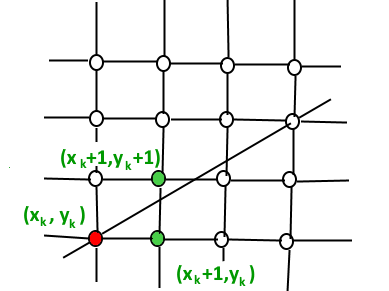
\includegraphics[scale=0.8]{BresenhamLine.png}
    \end{center}
    \caption{Bresenham problem}
    \label{fig:bresenham_problem}
\end{figure}

Hình \ref{fig:bresenham_problem} mô tả vấn đề cần giải quyết của thuật toán Bresenham: tại vị trí $x_k + 1$ cần chọn điểm $y_k$ hay $y_k+1$

\begin{figure}[H]
    \begin{center}
        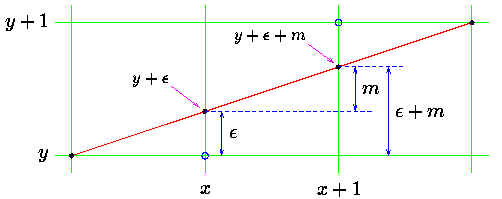
\includegraphics[scale=0.8]{bres1.png}
    \end{center}
    \caption{Digital differential analyzer (DDA)}
    \label{fig:dda_select}
\end{figure}

\begin{figure}[H]
    \begin{center}
        
\includegraphics[scale=0.5]{pseudo1.png}
    \end{center}
    \caption{Digital differential analyzer (DDA)}
    \label{fig:dda_algorithm}
\end{figure}

Giải sử:
\begin{itemize}
    \item $(x_1, y_1)$ là tọa độ điểm đầu.
    \item $(x_2, y_2)$ là tọa độ điểm cuối.
\end{itemize}

Trong trường hợp độ dốc của đường thẳng nằm trong đoạn từ 0 đến 1 và $x_1 <= x_2$, $y_1<y_2$, hình \ref{fig:dda_select} mô tả cách thuật toán DDA chọn điểm $y$ tiếp theo. Hình \ref{fig:dda_algorithm} là mã giả của thuật toán DDA. Ta thấy thuật toán có sử dụng các phép toán thập phân. Thuật toán Bresenham nâng cấp thuật toán DDA sao cho các phép toán của thuật toán thực hiện trên tập số nguyên.

\begin{figure}[H]
    \begin{center}
        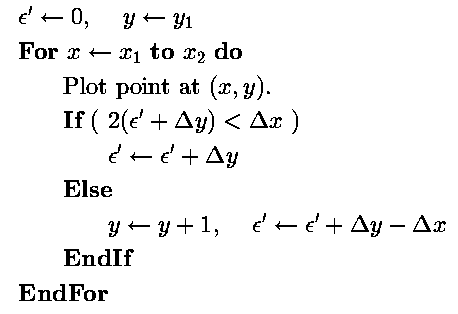
\includegraphics[scale=0.5]{pseudo2.png}
    \end{center}
    \caption{Bresenham Algorithm}
    \label{fig:bresenham_algorithm}
\end{figure}

Hình \ref{fig:bresenham_algorithm} là mã giả của thuật toán Bresenham trong trường hợp độ dốc của đường thẳng nằm trong đoạn từ 0 đến 1 và $x_1 <= x_2$, $y_1<y_2$.

Trong đó:
\begin{itemize}
    \item $\Delta x = x_2 - x_1$
    \item $\Delta y = y_2 - y_1$
\end{itemize}

% https://www.cs.helsinki.fi/group/goa/mallinnus/lines/bresenh.html

\subsection*{Thuật toán ICP trên không gian 2 chiều}
Giả sử ta có hai tập $m$ điểm $l = \{l_i(x^l_i, y^l_i) | i = \overline{1...m} \}$ và $r = \{r_i(x^r_i, y^r_i) | i = \overline{1...m} \}$. Ta cần tìm một phép biến đổi để biến đổi các điểm từ tập $l$ sang tập $r$. 

Một cách tổng quát có thể biến đổi bất kì một điểm từ tập $l$ sang tập $r$ bằng các phép xoay, scale và tịnh tiến:
\begin{equation}
    \lambda R l_i + t = r_i
\end{equation}
Trong đó:
\begin{itemize}
    \item $\lambda \in \mathbb{R}$ là hệ số scale, $\lambda > 0$
    \item $R \in \mathbb{R}^{2 \times 2}$ là ma trân xoay. $R = \begin{pmatrix}
        \cos{\alpha} & -\sin{\alpha}\\
        \sin{\alpha} & \cos{\alpha}
    \end{pmatrix}$ với $\alpha \in \left[0, 2\pi\right] $
    \item $t$ là vector tịnh tiến: $t = (t_x, t_y)^T$
\end{itemize}

Trong hầu hết các bài toán thực tế, các phép biến đổi không thể biến đổi tập $l$ về tập $r$ một cách hoàn toàn, ta chỉ có thể tìm phép biến đổi tốt nhất. Việc tìm phép biến đổi đó được đưa về việc tối ưu hóa hàm sau:

\begin{equation}
    D = \sum_{i = 1}^{m} \Vert \lambda R l_i + t - r_i\Vert ^2
    \label{eqn:icp_problem}
\end{equation}

Ta sẽ giải quyết bài toán tối ưu trên bằng cách tuyến tính hóa nó và lặp để tìm kết quả tốt nhất.

Đặt:
\begin{equation}
\begin{split}
    \overline{l} = \frac{1}{m}\sum_{i = 1}^{m} l_i \\
    \overline{r} = \frac{1}{m}\sum_{i = 1}^{m} r_i  
\end{split}
\label{eqn:reduced_coordinate_bar}
\end{equation}

\begin{equation}
\begin{split}
    l^{\prime}_i = l_i - \overline{l} \\
    r^{\prime}_i = r_i - \overline{r} \\
\end{split}
\label{eqn:reduced_coordinate}
\end{equation}

Khi đó:

\begin{equation}
    \begin{split}
        \sum_{i = 1}^{m} l^{\prime}_i = 0 \\
        \sum_{i = 1}^{m} r^{\prime}_i = 0 
    \end{split}
    \label{eqn:reduced_coordinate_condition}
\end{equation}

Thay \ref{eqn:reduced_coordinate_bar} và \ref{eqn:reduced_coordinate}
 vào \ref{eqn:icp_problem}, ta có:

\begin{equation}
\begin{split}
    D &= \sum_{i = 1}^{m} \Vert \lambda R l_i + t - r_i \Vert ^2 \\
      &= \sum_{i = 1}^{m} \Vert \lambda R (l^{\prime}_i + \overline{l}) - (r^{\prime}_i + \overline{r}) + t_i \Vert ^2 \\
      &= \sum_{i = 1}^{m} \Vert \lambda R l^{\prime}_i - r^{\prime}_i + \lambda R \overline{l} - \overline{r} + t \Vert ^2 \\
\end{split}
\end{equation}

Đặt:
\begin{equation}
    t^{\prime} = \lambda R \overline{l} - \overline{r} + t
\end{equation}

Ta có:
\begin{equation}
    \begin{split}
        D &= \sum_{i = 1}^{m} \Vert \lambda R l^{\prime}_i - r^{\prime}_i + t^{\prime} \Vert ^2 \\
          &= \sum_{i = 1}^{m} \Vert \lambda R l^{\prime}_i - r^{\prime}_i \Vert ^2 + 2{t^{\prime}}^T\sum_{i = 1}^{m} ( \lambda R l^{\prime}_i - r^{\prime}_i ) + \sum_{i = 1}^{m}\Vert t^{\prime} \Vert^2
    \end{split}
\end{equation}

Từ \ref{eqn:reduced_coordinate_condition} suy ra:
\begin{equation}
    \begin{split}
        D &= \sum_{i = 1}^{m} \Vert \lambda R l^{\prime}_i - r^{\prime}_i \Vert ^2 + 2{t^{\prime}}^T(0-0) + m\Vert t^{\prime} \Vert^2 \\ 
          &=  \sum_{i = 1}^{m} \Vert \lambda R l^{\prime}_i - r^{\prime}_i \Vert ^2 + m\Vert t^{\prime} \Vert^2 \\
          &= D_0 + mD_1
    \end{split}
\end{equation}

Ta thấy:
\begin{equation}
    \begin{split}
        D_1 &= \Vert t^{\prime} \Vert^2 \geq 0
    \end{split}
\end{equation}

Dấu bằng xảy ra khi và chỉ khi:
\begin{equation}
    \begin{split}
        & t^{\prime} = 0 \\
        \Leftrightarrow & \lambda R \overline{l} - \overline{r} + t = 0 \\
        \Leftrightarrow &t = \overline{r} - \lambda R \overline{l} 
    \end{split}
\end{equation}
Như vậy ta đã tìm được phép tịnh tiến tốt nhất $t = \overline{r} - \lambda R \overline{l} $.

Lại thấy:
\begin{equation}
    \begin{split}
        D_0 &= \sum_{i = 1}^{m} \Vert \lambda R l^{\prime}_i - r^{\prime}_i \Vert ^2 \\
        &= \lambda \sum_{i = 1}^{m} \Vert \sqrt{\lambda} R l^{\prime}_i - \frac{1}{\sqrt{\lambda}}r^{\prime}_i \Vert ^2 \\
        &= \lambda (\lambda \sum_{i = 1}^{m} \Vert R l^{\prime}_i  \Vert ^2 - 2\sum_{i = 1}^{m}{r^{\prime}_i}^T R l^{\prime}_i + \frac{1}{\lambda} \sum_{i = 1}^{m}\Vert r^{\prime}_i \Vert^2)\\
        &= \lambda (\lambda \sum_{i = 1}^{m} \Vert l^{\prime}_i  \Vert ^2 - 2\sum_{i = 1}^{m}{r^{\prime}_i}^T R l^{\prime}_i + \frac{1}{\lambda} \sum_{i = 1}^{m}\Vert r^{\prime}_i \Vert^2)\\
        &= \lambda (\lambda a - 2b + \frac{1}{\lambda}c)
    \end{split}
\end{equation}

Ta thấy $D_0$ đặt giá trị nhỏ nhất khi và chỉ khi:
\begin{equation}
    \begin{split}
    & \lambda a = \frac{1}{\lambda}c \\
    \Leftrightarrow & \lambda^2 = \frac{c}{a} \\
    \Leftrightarrow & \lambda^2 = \frac{\sum_{i = 1}^{m}\Vert r^{\prime}_i \Vert^2}{\sum_{i = 1}^{m} \Vert l^{\prime}_i  \Vert ^2}\\
    \Leftrightarrow & \lambda = \sqrt{\frac{\sum_{i = 1}^{m}\Vert r^{\prime}_i \Vert^2}{\sum_{i = 1}^{m} \Vert l^{\prime}_i  \Vert ^2}}
    \end{split}
\end{equation}

Như vậy ta đã tìm được phép co dãn tốt nhất $ \lambda = \sqrt{\frac{\sum_{i = 1}^{m}\Vert r^{\prime}_i \Vert^2}{\sum_{i = 1}^{m} \Vert l^{\prime}_i  \Vert ^2}}$

Giả sử  $r^{\prime}_i = (r^x_i, r^y_i)$ và $l^{\prime}_i = (l^x_i, l^y_i)$. Để $D_0$ đạt giá trị nhỏ nhất thì $b$ phải đạt giá trị lớn nhất.
Ta có:
\begin{equation}
    \begin{split}
    b &= \sum_{i = 1}^{m}{r^{\prime}_i}^T R l^{\prime}_i \\
    &= \sum_{i = 1}^{m} 
        \begin{bmatrix}
            r^x_i & r^y_i
        \end{bmatrix}
        \begin{bmatrix}
            \cos{\alpha} & -\sin{\alpha}\\
            \sin{\alpha} & \cos{\alpha}
        \end{bmatrix}
        \begin{bmatrix}
            l^x_i \\ l^y_i
        \end{bmatrix}\\
    &= \sum_{i = 1}^{m}
        \begin{bmatrix}
            r^x_i & r^y_i
        \end{bmatrix}
        \begin{bmatrix}
            l^x_i\cos{\alpha} & - l^y_i\sin{\alpha}\\
            l^x_i\sin{\alpha} & l^y_i\cos{\alpha}
        \end{bmatrix}\\
    &= \sum_{i = 1}^{m} (\cos{\alpha}(r^x_i l^x_i + r^y_i l^y_i) + \sin{\alpha}(-r^x_i l^y_i + r^y_i l^x_i)) \\
    &= 
        \begin{bmatrix}
            \cos{\alpha} & \sin{\alpha}
        \end{bmatrix}
        \begin{bmatrix}
            \sum_{i = 1}^{m} (r^x_i l^x_i + r^y_i l^y_i) \\
            \sum_{i = 1}^{m} (-r^x_i l^y_i + r^y_i l^x_i)
        \end{bmatrix}
    \end{split}
\end{equation}

$b$ đạt giá trị lớn nhất khi và chỉ khi:
\begin{equation}
    \begin{bmatrix}
        \cos{\alpha} \\ \sin{\alpha}
    \end{bmatrix}
    == \frac{1}{\Vert P \Vert^2}P
\end{equation}
Với:
\begin{equation}
    P = 
    \begin{bmatrix}
        \sum_{i = 1}^{m} (r^x_i l^x_i + r^y_i l^y_i) \\
        \sum_{i = 1}^{m} (-r^x_i l^y_i + r^y_i l^x_i)
    \end{bmatrix}
\end{equation}
Như vậy ta cũng đã tìm được phép xoay tốt nhất $R$.
Sau khi đã tìm được 3 phép biến đổi $(\lambda, R, t)$, ta áp dụng phép biến đổi này vào cho vị trí của robot sẽ được vị trí mới. Tiếp tục tìm điểm tương ứng nhờ thuật toán Bresenham, với bộ điểm tương ứng đó ta sẽ có một bộ phép biến đổi $(\lambda, R, t)$ mới để áp dụng vào vị trí của robot. Thuật toán dừng lại cho đến khi phép biến đổi gần như không thay đổi vị trí robot hoặc qua một số vòng lặp nhất định. Hình \ref{fig:icp} mô tả kết quả mong muốn đạt được khi sử dụng thuật toán ICP.

\begin{figure}[H]
    \begin{center}
        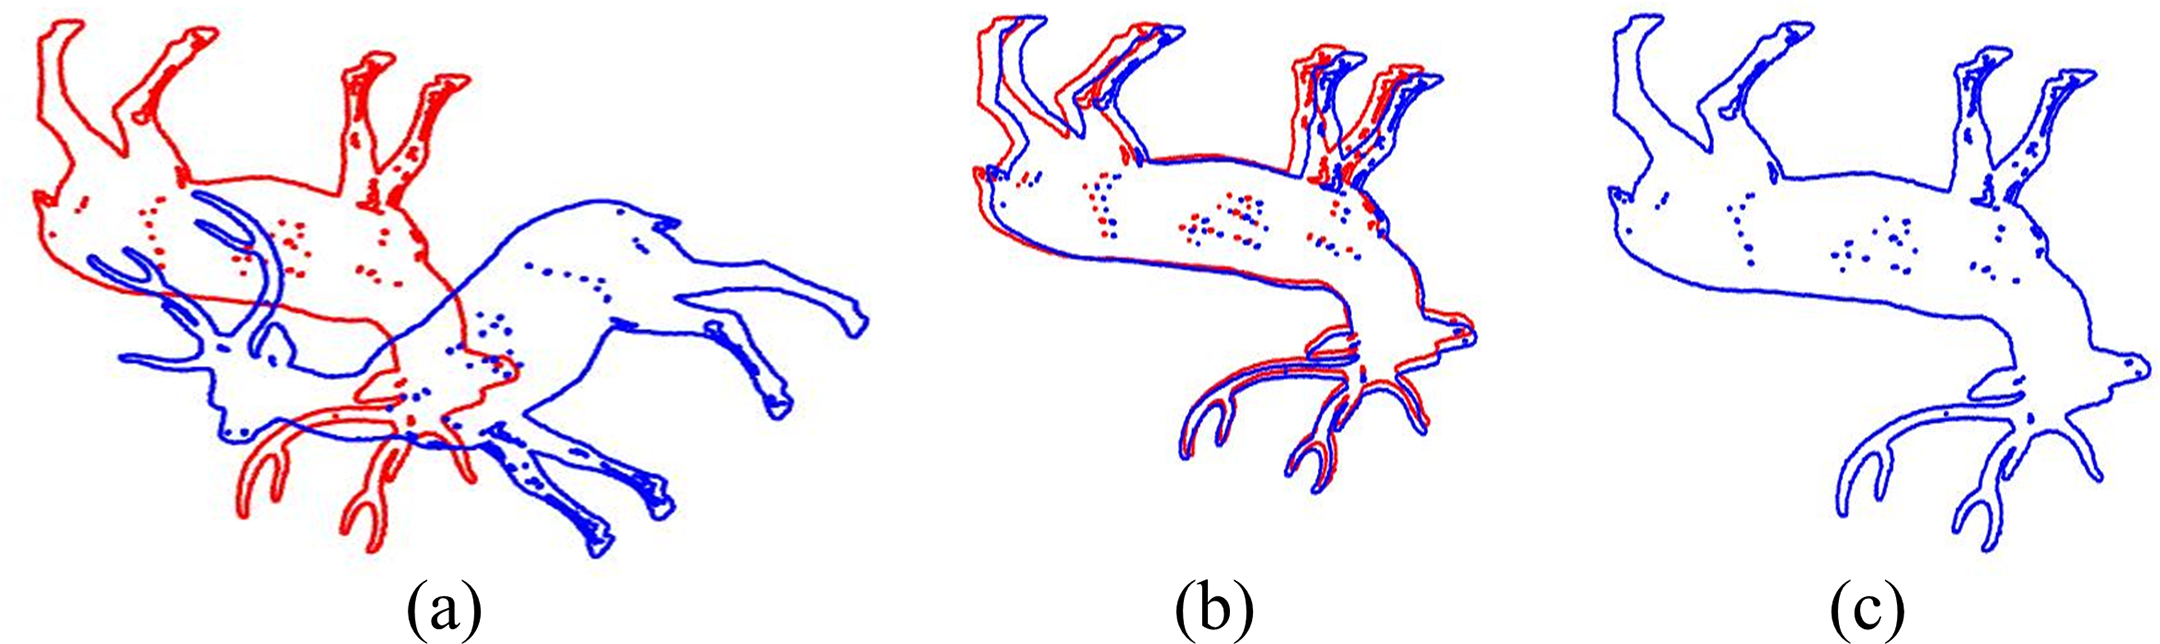
\includegraphics[scale=0.6]{icp.png}
    \end{center}
    \caption{ICP algorithm demonstation}
    \label{fig:icp}
\end{figure}

\section{Tính weight cho từng particle - Scoring}
Với mỗi particle, ta tính weight dựa vào sự tương đồng giữa các điểm cuối tính từ ranging data và vị trí của robot so với các điểm tương ứng trên map. Việc tìm điểm tương đồng sử dụng thuật toán Bresenham.

Giả sử  ta có $M$ điểm cuối $(x_i^r, y_i^r)^T$ và $M$ điểm tương ứng trên map $(x_i^m, y_i^m)^T$, weight cho mỗi particle được tính theo công thức:
\begin{equation}
    w_i = \frac{m}{\exp((x_i^r-x_i^m)^2 + (y_i^r - y_i^m)^2)}
\end{equation}
Với $m$ là xác suất mà ô có vị trí $(x_i^m, y_i^m)^T$ trên map bị chiếm dụng.

\section{Lấy mẫu lại - Resampling}
Việc lấy mẫu lại có mục đích làm tăng sự xuất hiện của các particle có weight cao đồng thời làm giảm hoặc biến mất các particle có trọng số thấp.
Thuật toán multinomial resampling được sử dụng để lấy mẫu lại các particle.

\begin{figure}[H]
    \begin{center}
        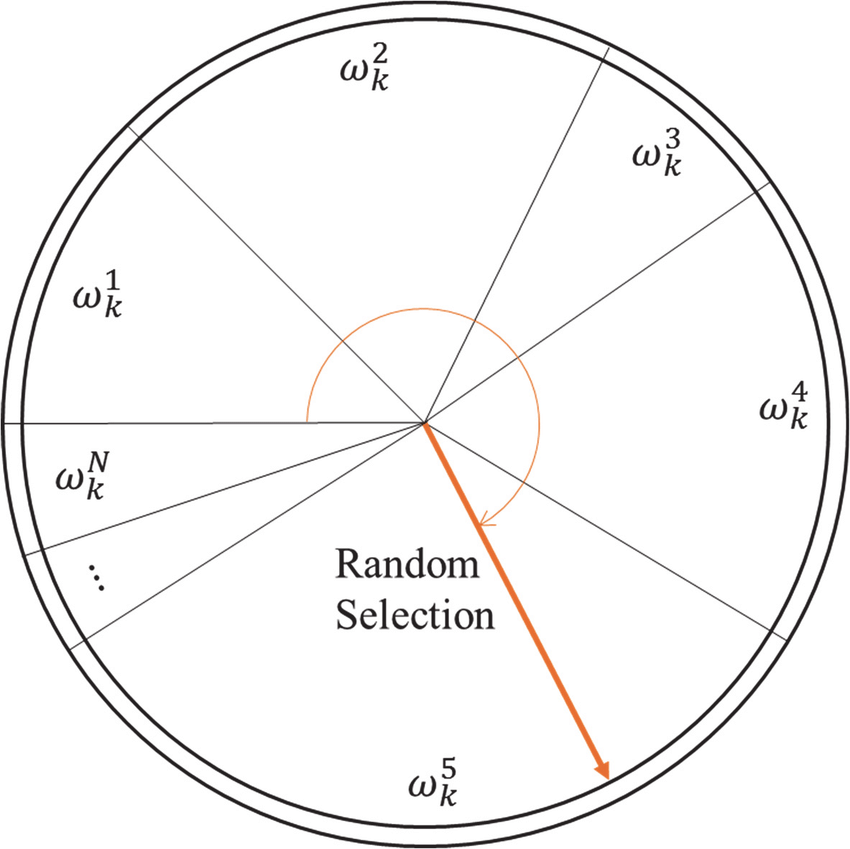
\includegraphics[scale=0.2]{Visualization-of-multinomial-resampling-algorithm.png}
    \end{center}
    \caption{Mô tả hình học của thuật toán multinomial resampling}
    \label{fig:Visualization-of-multinomial-resampling-algorithm}
\end{figure}

Multinomial resampling bao gồm các bước sau:
\begin{itemize}
    \item Chuẩn hóa cái giá trị weight
    \item Tính tổng tính lũy các weight
    \item Lấy mẫu ngẫu nhiên $N$ số  có khoảng giá trị từ 0 đến 1 theo phân phối đều
    \item Với mỗi mẫu lấy được, xác định vị trí của weight mà nó thuộc về và lấy mẫu particle tương ứng với weight đó. VD: trong hình \ref{fig:Visualization-of-multinomial-resampling-algorithm}, mẫu màu cam nằm trong vị trí của $w^5$ nên particle có weight là $w^5$ được lấy mẫu.
\end{itemize}

\section{Cập nhật lại map - Map update}

\begin{figure}[H]
    \begin{center}
        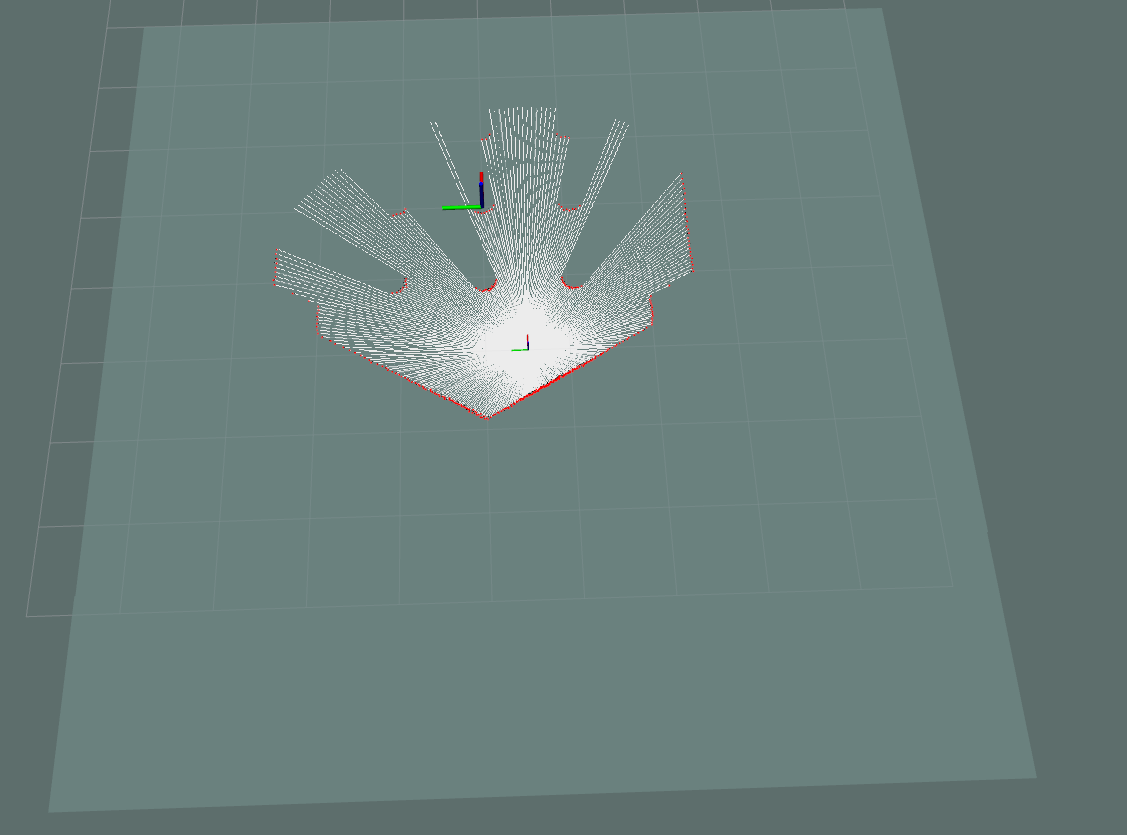
\includegraphics[scale=0.3]{map_update.png}
    \end{center}
    \caption{Map update}
    \label{fig:map_update}
\end{figure}

Sau bước resmapling, chỉ còn các particle tốt nhất ở lại. Khi đó, ta có thể tự tin với vị trí hiện tại của robot nên quá trình cập nhật map có thể được tiến hành.

Để cập nhập map, thuật toán Bresenham được sử dụng để update một local map, sau đó local map sẽ được update vào global map. Điều này được thể hiện trong hình \ref{fig:map_update}.

\section{Thực hiện các bước bằng tính toán song song}.

Bằng cách xem xét các bước của GMapping, ta thấy nhiều bước có thể  được thực hiện song song, cụ thể là:
\begin{itemize}
    \item Prediction: Bước này sẽ chạy song song cho các particle.
    \item Correction: Thuật toán ICP sẽ chạy song song cho từng particle. Trong mỗi particle , thuật toán Bresenham sẽ chạy song song cho từng beam của laser.
    \item Resampling: Bước này sẽ chạy nối tiếp.
    \item Map update: Bước này sẽ chạy song song cho từng particle.
\end{itemize}

\end{document}